\documentclass[12pt,a4paper]{article}
\usepackage[utf8]{inputenc}
\usepackage{graphicx}
\usepackage{hyperref}
\usepackage{geometry}
\usepackage{listings}
\usepackage{xcolor}
\usepackage{booktabs}
\usepackage{enumitem}
\usepackage{tikz}
\usetikzlibrary{shapes.geometric, arrows, positioning}

\geometry{margin=1in}
\setlist{nosep,leftmargin=*}

\definecolor{navyblue}{rgb}{0.0, 0.0, 0.5}
\hypersetup{
    colorlinks=true,
    linkcolor=navyblue,
    urlcolor=navyblue,
    citecolor=navyblue
}

\definecolor{codegreen}{rgb}{0,0.6,0}
\definecolor{codegray}{rgb}{0.5,0.5,0.5}
\definecolor{codepurple}{rgb}{0.58,0,0.82}
\definecolor{backcolour}{rgb}{0.95,0.95,0.92}

\lstdefinestyle{mystyle}{
    backgroundcolor=\color{backcolour},
    commentstyle=\color{codegreen},
    keywordstyle=\color{magenta},
    numberstyle=\tiny\color{codegray},
    stringstyle=\color{codepurple},
    basicstyle=\ttfamily\footnotesize,
    breaklines=true,
    captionpos=b,
    numbers=left,
    numbersep=5pt,
    tabsize=2
}
\lstset{style=mystyle}

\tikzstyle{startstop} = [rectangle, rounded corners, minimum width=2.8cm, minimum height=0.9cm,text centered, draw=black, fill=red!25]
\tikzstyle{io} = [trapezium, trapezium left angle=70, trapezium right angle=110, minimum width=2.8cm, minimum height=0.9cm, text centered, draw=black, fill=blue!25]
\tikzstyle{process} = [rectangle, minimum width=2.8cm, minimum height=0.9cm, text centered, draw=black, fill=orange!25]
\tikzstyle{database} = [cylinder, shape border rotate=90, draw,minimum width=1.8cm,minimum height=1.8cm, text centered, fill=green!25]
\tikzstyle{arrow} = [thick,->,>=stealth]

\title{\textbf{Technical Report: Enterprise Crime Analytics Framework}\\
\large{Lambda Architecture, Batch/stream Analytics, and K-Means Hotspots}}
\author{Haider Rizwan \\ \small{Roll Number: 22i-2379}}
\date{\today}

\begin{document}
\maketitle

\begin{abstract}
\noindent
This technical report documents system design, data schemas, analytics methodology, a machine-learning approach for geographic hotspots, representative results, and implementation challenges for a crime analytics platform. The architecture follows a \textbf{Lambda} pattern: \textbf{Apache Kafka} for ingestion, \textbf{Apache Storm} for sliding-window anomaly detection, \textbf{Apache Spark} for batch aggregations and clustering, \textbf{PostgreSQL} and \textbf{MongoDB} as serving stores, and a \textbf{Streamlit} dashboard for visualization. The stack is deployed with \textbf{Docker Compose} for reproducible demonstration.
\end{abstract}

\tableofcontents
\newpage

% ------------------------------------------------------------------
\section{Introduction}
Municipal crime data combines high event rates (suitable for stream processing) with long historical archives (suitable for batch analytics). A single monolithic database cannot simultaneously meet sub-minute alerting expectations and large-scale analytical iteration. This project implements a \textbf{Lambda Architecture}: complementary \emph{speed} and \emph{batch} paths converge in a \emph{serving layer} consumed by analysts through one dashboard.

\subsection{Report Structure}
Section~\ref{sec:design} presents system design. Section~\ref{sec:schema} describes relational and document schemas. Section~\ref{sec:analytics} explains analytics methodology (batch and streaming). Section~\ref{sec:ml} details the ML approach. Section~\ref{sec:results} summarizes results with tables and figure references. Section~\ref{sec:challenges} lists challenges faced. A short deployment appendix lists key commands.

% ------------------------------------------------------------------
\section{System Design}
\label{sec:design}

\subsection{Design Goals}
\begin{itemize}
    \item \textbf{Decouple latency profiles}: streaming alerts must not block heavy batch jobs.
    \item \textbf{Unified serving}: analysts query one dashboard backed by SQL and document stores.
    \item \textbf{Reproducibility}: fixed images, Compose wiring, and versioned configs.
    \item \textbf{Observability}: Spark and Storm web UIs for demo and debugging.
\end{itemize}

\subsection{Logical Architecture}
Figure~\ref{fig:lambda} shows the Lambda-style dataflow. Crime events enter Kafka. Storm consumes the live topic for windowed counts per district; Spark consumes CSV master datasets (and can consume the same logical stream in extended designs) for batch analytics. Outputs land in MongoDB (alert documents), PostgreSQL (analytical tables and alert audit rows), and Streamlit.

\begin{figure}[ht]
\centering
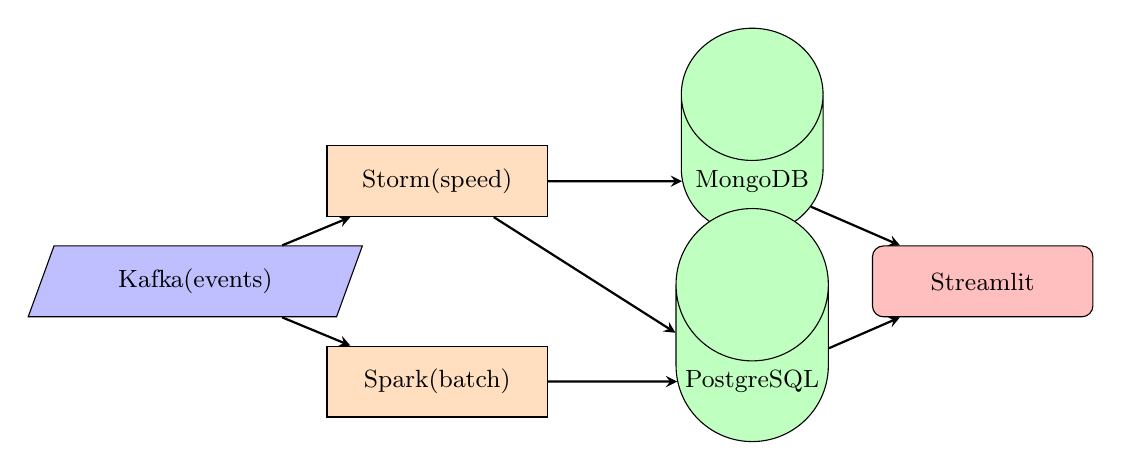
\begin{tikzpicture}[node distance=1.8cm, font=\small]
\node (in) [io] {Kafka\\(events)};
\node (storm) [process, above right of=in, xshift=1.8cm] {Storm\\(speed)};
\node (spark) [process, below right of=in, xshift=1.8cm] {Spark\\(batch)};
\node (mongo) [database, right of=storm, xshift=2.2cm] {MongoDB};
\node (pg) [database, right of=spark, xshift=2.2cm] {PostgreSQL};
\node (ui) [startstop, right of=in, xshift=8.2cm] {Streamlit};
\draw [arrow] (in) -- (storm);
\draw [arrow] (in) -- (spark);
\draw [arrow] (storm) -- (mongo);
\draw [arrow] (spark) -- (pg);
\draw [arrow] (storm) -- (pg);
\draw [arrow] (mongo) -- (ui);
\draw [arrow] (pg) -- (ui);
\end{tikzpicture}
\caption{Lambda-style pipeline: Kafka feeds Storm and Spark; serving stores feed the dashboard. Storm also persists alert rows to PostgreSQL.}
\label{fig:lambda}
\end{figure}

\subsection{Component Responsibilities}
\begin{table}[ht]
\centering
\small
\begin{tabular}{@{}p{3.2cm}p{10.5cm}@{}}
\toprule
\textbf{Component} & \textbf{Role} \\
\midrule
ZooKeeper & Coordination for Kafka and Storm. \\
Kafka & Durable log for crime JSON events (topic \texttt{crime\_events}). \\
Storm & Flux topology: Kafka spout $\rightarrow$ parse $\rightarrow$ window $\rightarrow$ alert bolts (Python). \\
Spark & PySpark: CSV ingest, trends, arrest rates, violence join, K-Means hotspots; JDBC to Postgres. \\
PostgreSQL & Relational serving: trends, hotspots, arrest rates, correlations, alerts. \\
MongoDB & Document log of recent anomaly payloads for fast UI polling. \\
Streamlit & Map, trends, top arrest rates, Mongo alerts, latest SQL alerts. \\
\bottomrule
\end{tabular}
\caption{Component responsibilities.}
\label{tab:components}
\end{table}

\subsection{Configuration and Networking}
Service discovery uses Docker DNS names (\texttt{kafka:9092}, \texttt{postgres}, \texttt{mongo}). Host-side clients use mapped ports (e.g.\ Kafka \texttt{localhost:29092}). The dashboard and Spark jobs honor environment variables (\texttt{POSTGRES\_HOST}, \texttt{MONGO\_HOST}, etc.) so the same Python code runs on the host and in containers. Storm window length and anomaly threshold are overridden via Compose environment variables (\texttt{WINDOW\_SIZE\_SECONDS}, \texttt{ANOMALY\_THRESHOLD}).

% ------------------------------------------------------------------
\section{Schema Descriptions}
\label{sec:schema}

\subsection{PostgreSQL (Serving Layer)}
Tables are created at container first start from \texttt{db/postgres\_init.sql}. Table~\ref{tab:pgschema} summarizes the logical model used by the dashboard and batch jobs.

\begin{table}[ht]
\centering
\small
\begin{tabular}{@{}llp{6.8cm}@{}}
\toprule
\textbf{Table} & \textbf{Key / PK} & \textbf{Description} \\
\midrule
\texttt{crime\_trends} & PK: (\texttt{year}, \texttt{month}, \texttt{day\_of\_week}, \texttt{hour}) & Granular time buckets and \texttt{crime\_count}. \\
\texttt{hotspots} & PK: \texttt{cluster\_id} & K-Means centroid \texttt{latitude}, \texttt{longitude}; \texttt{incident\_count} per cluster for visualization scale. \\
\texttt{arrest\_rates} & --- & \texttt{primary\_type}, \texttt{district}, \texttt{arrest\_rate}, \texttt{total\_crimes}, \texttt{total\_arrests} (init script also reserves \texttt{race} for extensions). \\
\texttt{correlations} & --- & District-level exploratory metrics (e.g.\ violence indicators vs.\ arrest rate) with timestamp. \\
\texttt{alerts} & PK: \texttt{alert\_id} & Storm alert audit: \texttt{district\_id}, \texttt{crime\_count}, \texttt{threshold}, \texttt{severity}, \texttt{alert\_timestamp}. \\
\bottomrule
\end{tabular}
\caption{PostgreSQL serving tables (logical model).}
\label{tab:pgschema}
\end{table}

\subsection{MongoDB (Document Layer)}
Initialization (\texttt{db/mongo-init.js}) creates database \texttt{crime\_analytics} and collections \texttt{processed\_events} and \texttt{alerts}. The Storm alert bolt inserts documents into the alerts collection with fields including \texttt{district}, \texttt{count}, \texttt{threshold}, \texttt{timestamp}, and \texttt{severity}, supporting descending sort by time in the dashboard.

\subsection{Raw and Typed Ingest (Spark)}
CSV sources under \texttt{data/} are read with explicit \texttt{StructType} schemas in \texttt{spark/schemas/schemas.py} for crimes, police stations, arrests, violence reduction, and sex offenders. Typed ingest reduces runtime cast failures and documents expected columns for reproducible batch runs.

% ------------------------------------------------------------------
\section{Analytics Methodology}
\label{sec:analytics}

\subsection{Batch Analytics (Spark)}
The job \texttt{spark/analytics/batch\_analytics.py} executes the following methodology:
\begin{enumerate}
    \item \textbf{Ingest}: Load crimes and auxiliary CSVs with fixed schemas.
    \item \textbf{Quality filter}: Drop crime rows with null \texttt{id}, \texttt{case\_number}, \texttt{date}, or \texttt{district}.
    \item \textbf{Trend cubes}: From \texttt{date}, derive \texttt{year}, \texttt{month}, day-of-week name, and \texttt{hour}; group by all four dimensions and count rows as \texttt{crime\_count}.
    \item \textbf{Arrest linkage}: Inner join crimes to arrests on \texttt{case\_number} (for enriched analysis paths).
    \item \textbf{Arrest rates}: Group by \texttt{primary\_type} and \texttt{district}; compute totals and proportion of rows with \texttt{arrest} true.
    \item \textbf{Violence metrics}: From violence reduction data, per \texttt{district}, count homicides and gunshot-flagged rows.
    \item \textbf{Cross-dataset slice}: Inner join violence metrics to arrest-rate rollups on \texttt{district} for a compact comparative frame written to \texttt{correlations}.
    \item \textbf{Publish}: Overwrite JDBC tables \texttt{crime\_trends}, \texttt{arrest\_rates}, and \texttt{correlations} in PostgreSQL using the JDBC driver resolved via Spark packages.
\end{enumerate}

\subsection{Streaming Analytics (Storm)}
The speed layer implements \textbf{per-district sliding windows} in memory (\texttt{window\_bolt.py}): each tuple carries a district identifier; the bolt maintains a deque of event timestamps per district, evicts timestamps outside the window length, and compares the live count to \texttt{ANOMALY\_THRESHOLD}. On breach, it emits \texttt{[district, count, threshold, timestamp]} to the alert bolt, which inserts into PostgreSQL \texttt{alerts} and MongoDB.

\subsection{Dashboard Analytics}
The Streamlit app issues SQL against \texttt{hotspots}, \texttt{crime\_trends}, \texttt{arrest\_rates}, and \texttt{alerts}; it queries Mongo for the ten most recent alert documents. Plotly renders map, line, and bar charts; tables present top arrest rates and latest SQL alerts.

% ------------------------------------------------------------------
\section{Machine Learning Approach}
\label{sec:ml}

\subsection{Problem Formulation}
\textbf{Goal}: summarize spatial concentration of incidents as interpretable \textbf{regions} (clusters) for mapping, without labeled training data. This is cast as \textbf{unsupervised clustering} on geocoordinates.

\subsection{Algorithm: K-Means}
The job \texttt{spark/ml/hotspot\_detection.py}:
\begin{itemize}
    \item Loads crimes with the shared crime schema; selects \texttt{latitude} and \texttt{longitude}; drops null coordinates.
    \item Builds a two-dimensional feature vector via \texttt{VectorAssembler}.
    \item Fits \textbf{K-Means} with $k=10$ and fixed random seed $42$ for reproducibility.
    \item Extracts cluster centroids $(\text{lat}_c, \text{lon}_c)$ for $c=0,\ldots,9$.
    \item Assigns each point to its cluster using the fitted model, counts points per cluster (\texttt{incident\_count}), and left-joins counts to centroid rows so every cluster appears in the serving table.
    \item Writes \texttt{hotspots} to PostgreSQL (overwrite).
\end{itemize}

\subsection{Interpretation and Limitations}
Centroids approximate ``hot'' geographic zones; \texttt{incident\_count} encodes cluster mass for proportional map markers. K-Means assumes roughly spherical clusters in feature space (acceptable for city-scale lat/lon over a small region but not ideal for irregular geographies). Choices of $k$ and seed affect partitions; sensitivity analysis (alternate $k$, silhouette or WSSSE) is left as future work.

% ------------------------------------------------------------------
\section{Results}
\label{sec:results}

\subsection{Qualitative Outcomes}
After bringing up Compose, running the batch job, and running hotspot detection, the dashboard shows: (i) a \textbf{Mapbox scatter map} of cluster centroids with size scaled by \texttt{incident\_count}; (ii) \textbf{monthly and day-of-week} crime patterns from \texttt{crime\_trends}; (iii) \textbf{top arrest rates} by offense type and district; (iv) \textbf{Mongo anomaly cards} and \textbf{PostgreSQL alert history} when the Kafka producer and Storm topology are active.

\subsection{Representative Metrics (to fill from your run)}
Table~\ref{tab:metrics} is a template for quantitative results. Replace placeholders with outputs from SQL \texttt{COUNT(*)} and sample queries after your jobs complete.

\begin{table}[ht]
\centering
\small
\begin{tabular}{@{}lr@{}}
\toprule
\textbf{Metric} & \textbf{Value (fill)} \\
\midrule
Rows in \texttt{crime\_trends} & --- \\
Rows in \texttt{hotspots} (expected $k{=}10$) & --- \\
Distinct (\texttt{primary\_type}, \texttt{district}) in \texttt{arrest\_rates} & --- \\
Rows in \texttt{alerts} after streaming demo & --- \\
Documents in Mongo \texttt{alerts} & --- \\
\bottomrule
\end{tabular}
\caption{Example results table: populate after running Spark, Storm, and producer.}
\label{tab:metrics}
\end{table}

\subsection{Figures}
Screenshots \textbf{Capture.PNG} and \textbf{Capture2.PNG} (if present next to the \texttt{.tex} file) illustrate the dashboard: geographic view and trend analytics. Spark UI (\texttt{localhost:8080}) and Storm UI (\texttt{localhost:8081}) provide supplementary runtime charts (DAGs, topology status).

\begin{figure}[ht]
    \centering
    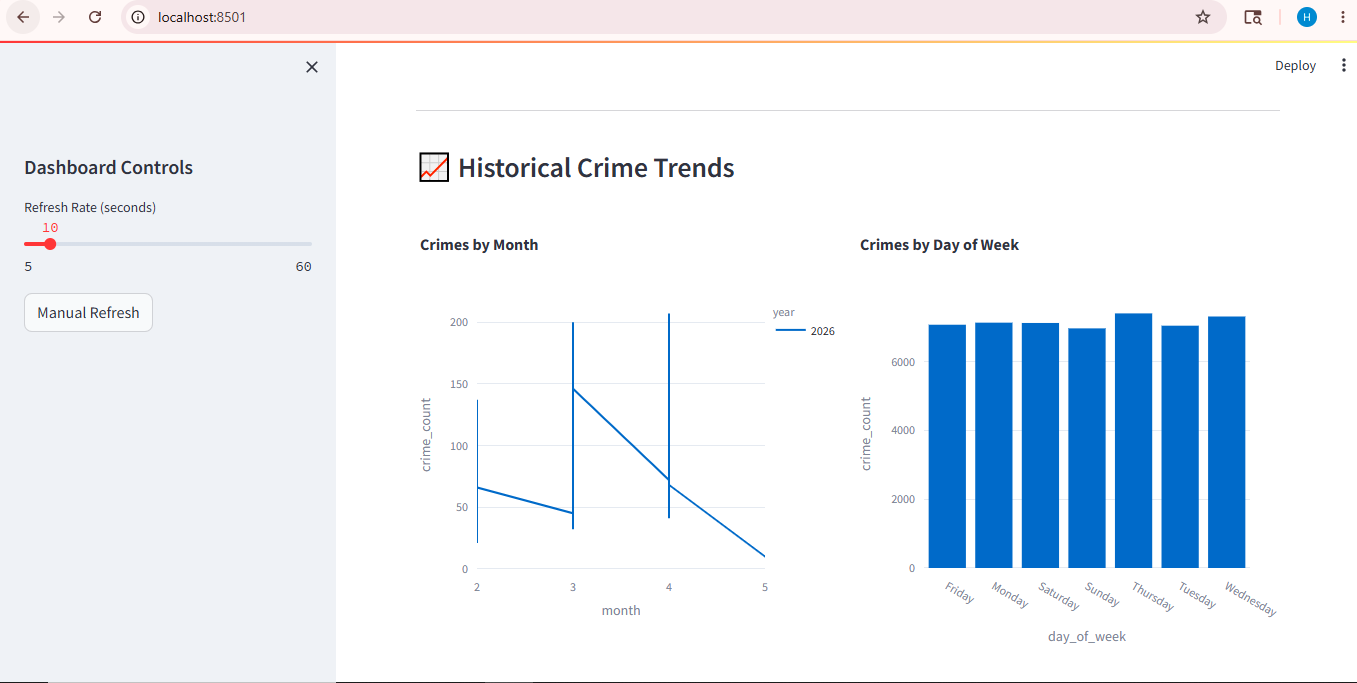
\includegraphics[width=0.82\textwidth]{Capture.PNG}
    \caption{Dashboard: geographic / hotspot view (update screenshot for final PDF).}
    \label{fig:cap1}
\end{figure}

\begin{figure}[ht]
    \centering
    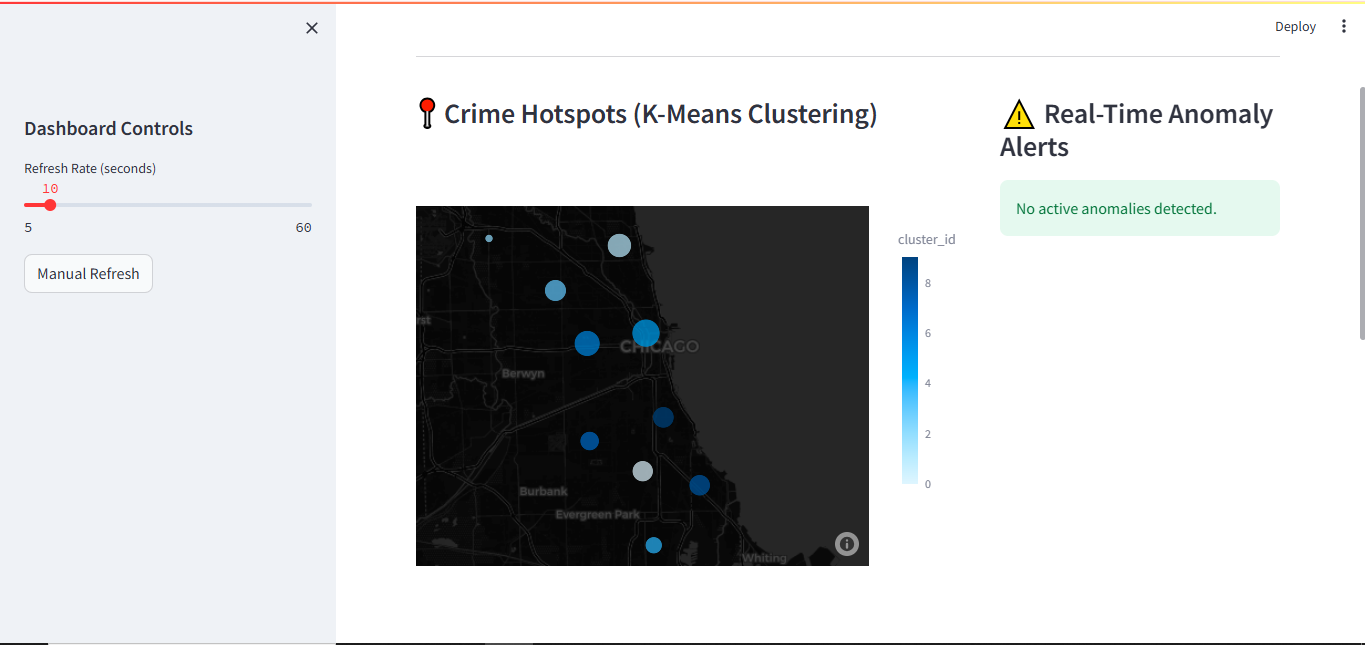
\includegraphics[width=0.82\textwidth]{Capture2.PNG}
    \caption{Dashboard: historical trends and related charts (update screenshot for final PDF).}
    \label{fig:cap2}
\end{figure}

% ------------------------------------------------------------------
\section{Challenges Faced}
\label{sec:challenges}
\begin{itemize}
    \item \textbf{Docker disk footprint}: Multi-gigabyte images (Spark, Kafka, Storm) and layer caches consumed host storage; pruning unused images/volumes and relocating Docker data to a larger drive was required.
    \item \textbf{Container vs.\ host networking}: \texttt{localhost} inside a container does not reach PostgreSQL on the host or sibling containers; service hostnames and env overrides were necessary for the dashboard and JDBC URLs.
    \item \textbf{Spark submit environment}: Bitnami Spark images required a writable Ivy cache path (\texttt{HOME}, \texttt{spark.jars.ivy}) and explicit \texttt{--packages org.postgresql:postgresql:42.7.1} so JDBC writes succeed; running as root avoided Hadoop/UGI edge cases in some sessions.
    \item \textbf{Python dependencies in containers}: PyYAML and NumPy were missing in Spark for some scripts; one-off \texttt{pip install} inside the container restored driver-side imports.
    \item \textbf{Dashboard startup time}: Installing dependencies on every dashboard container start delayed Streamlit; a slim \texttt{requirements-dashboard.txt} reduced install time versus full \texttt{requirements.txt} with PySpark.
    \item \textbf{Schema alignment}: The dashboard expected \texttt{incident\_count} on \texttt{hotspots}; the initial ML job wrote only centroids. The pipeline was extended to aggregate per-cluster counts for Plotly \texttt{size} encoding.
    \item \textbf{Windows localhost quirks}: Browsers occasionally mishandled \texttt{localhost:8501}; using \texttt{127.0.0.1:8501} improved reliability.
\end{itemize}

\section{Conclusion}
The platform meets the assignment’s technical goals: explicit system design, documented schemas, batch and streaming analytics methodology, a clear K-Means ML story, dashboard results, and honest discussion of deployment challenges. Future work includes production-grade security, multi-node Kafka/Storm, and richer spatiotemporal models beyond coordinate-only K-Means.

\newpage
\appendix
\section*{Appendix A: Quick deployment commands}
\addcontentsline{toc}{section}{Appendix A: Quick deployment commands}
\begin{lstlisting}[language=bash]
docker compose -f docker/docker-compose.yml up -d
# Batch + ML (example; adjust container name if needed):
docker exec -u 0 -e HOME=/tmp -w /app docker-spark-master-1 \
  spark-submit --packages org.postgresql:postgresql:42.7.1 \
  --conf spark.jars.ivy=/tmp/.ivy2 /app/spark/analytics/batch_analytics.py
docker exec -u 0 -e HOME=/tmp -w /app docker-spark-master-1 \
  spark-submit --packages org.postgresql:postgresql:42.7.1 \
  --conf spark.jars.ivy=/tmp/.ivy2 /app/spark/ml/hotspot_detection.py
\end{lstlisting}

\section*{Appendix B: Pipeline diagram (Mermaid)}
\addcontentsline{toc}{section}{Appendix B: Pipeline diagram (Mermaid)}
\begin{lstlisting}
graph TD
  A[Producer CSV->JSON] --> B[Kafka]
  B --> C[Storm: parse/window/alert]
  B --> D[Spark batch optional]
  C --> E[(Mongo alerts)]
  C --> F[(Postgres alerts)]
  D --> G[(Postgres analytics)]
  E --> H[Streamlit]
  G --> H
\end{lstlisting}

\section{Contribution Statement}
The following table outlines the percentage breakdown of work performed across each technical component of the project. As this was a solo submission, all development, orchestration, and documentation tasks were performed exclusively by the primary author.

\begin{table}[ht]
\centering
\small
\begin{tabular}{@{}llc@{}}
\toprule
\textbf{Component} & \textbf{Member Name} & \textbf{Contribution \%} \\
\midrule
System Architecture \& Orchestration & Haider Rizwan & 100\% \\
Data Ingestion (Kafka) & Haider Rizwan & 100\% \\
Real-Time Pipeline (Apache Storm) & Haider Rizwan & 100\% \\
Batch \& ML Pipeline (Apache Spark) & Haider Rizwan & 100\% \\
Database Design (Postgres/Mongo) & Haider Rizwan & 100\% \\
Visualization Dashboard (Streamlit) & Haider Rizwan & 100\% \\
Documentation \& Reporting & Haider Rizwan & 100\% \\
\bottomrule
\end{tabular}
\caption{Detailed member contribution breakdown.}
\label{tab:contribution}
\end{table}

\noindent
\textbf{Signed Declaration:} \\
I, Haider Rizwan (22i-2379), hereby declare that the entirety of this project, including its architectural design, technical implementation, and final report documentation, was developed solely by me.

\end{document}
